\section{Tuần 5: Thuật toán Vẽ Đường cong Ellipse, Đường cong Bézier và Phân vùng Đa giác}
\label{sec:week5}

\subsection{Thuật toán Vẽ Cung tròn và Cung Ellipse trên Lưới Tọa độ Nguyên}
\label{subsec:w5_arc}

Trong đồ họa máy tính, việc tạo dựng các đường cong bậc hai (Conic Sections) như cung tròn và ellipse đòi hỏi các giải pháp rời rạc hóa tối ưu nhằm xác định chính xác các điểm ảnh nguyên trên màn hình hiển thị~\citep{hearn2004computer,foley1996computer}.

\textbf{1. Kỹ thuật Vẽ Cung tròn (Circular Arc Generation):}
Khác với đường tròn khép kín hoàn chỉnh vốn tận dụng triệt để tính đối xứng 8 phần để sinh toàn bộ chu vi từ một cung bát phân đơn lẻ, việc vẽ một cung tròn giới hạn bởi góc xuất phát $\theta_{\text{start}}$ và góc kết thúc $\theta_{\text{end}}$ (với $\theta \in [0, 2\pi]$) đòi hỏi cơ chế kiểm tra điều kiện góc hoặc tọa độ mút:
\begin{itemize}
    \item \textit{Phương pháp góc cực:} Thuật toán Midpoint Circle duyệt qua các điểm ứng viên, sau đó tính góc cực $\theta = \text{atan2}(y - y_c, x - x_c)$ (hoặc dùng phép so sánh tích vô hướng và tích có hướng giữa vector hiện tại với hai vector giới hạn biên mút). Điểm ảnh chỉ được xuất ra bộ đệm khung hình (Frame Buffer) nếu góc nằm trong khoảng $[\theta_{\text{start}}, \theta_{\text{end}}]$.
    \item \textit{Phương pháp điểm mút:} Xác định trước tọa độ nguyên của hai điểm đầu mút $P_{\text{start}}(x_s, y_s)$ và $P_{\text{end}}(x_e, y_e)$ trên đường tròn giải tích, sau đó chạy giải thuật gia số dọc theo chiều quay xác định và dừng vòng lặp khi chạm tới điểm mút kết thúc.
\end{itemize}

\textbf{2. Thuật toán Vẽ Đường cong Ellipse Điểm Giữa (Midpoint Ellipse Algorithm):}
Phương trình đại số của một hình ellipse chuẩn có tâm tại gốc tọa độ $O(0, 0)$ với bán trục lớn $r_x$ dọc theo trục hoành và bán trục nhỏ $r_y$ dọc theo trục tung có dạng:
\begin{equation}
\frac{x^2}{r_x^2} + \frac{y^2}{r_y^2} = 1
\end{equation}
Khử mẫu số, ta định nghĩa hàm ellipse giải tích:
\begin{equation}
f_{\text{ellipse}}(x, y) = r_y^2 x^2 + r_x^2 y^2 - r_x^2 r_y^2
\end{equation}
với dấu của hàm phân định vị trí tương đối: $f_{\text{ellipse}}(x, y) < 0$ khi điểm nằm trong ellipse, $f_{\text{ellipse}}(x, y) = 0$ khi điểm nằm trên biên, và $f_{\text{ellipse}}(x, y) > 0$ khi điểm nằm ngoài ellipse.

Hình ellipse đối xứng qua hai trục tọa độ $x = 0$ và $y = 0$, do đó chỉ cần khảo sát trong góc phần tư thứ nhất ($x \ge 0, y \ge 0$), sau đó áp dụng tính đối xứng 4 phần (4-Way Symmetry) để suy ra các điểm trên 3 góc phần tư còn lại:
\begin{equation}
(x, y), \quad (-x, y), \quad (x, -y), \quad (-x, -y)
\end{equation}

Khác với đường tròn có độ cong đồng đều, độ dốc tiếp tuyến của ellipse thay đổi liên tục:
\begin{equation}
\frac{dy}{dx} = -\frac{r_y^2 x}{r_x^2 y}
\end{equation}
Do đó, góc phần tư thứ nhất được phân tách thành hai miền rõ rệt thông qua điểm phân giới có độ lớn độ dốc bằng $1$ ($|\frac{dy}{dx}| = 1 \iff 2 r_y^2 x = 2 r_x^2 y$):

\textbf{Miền 1 (Region 1: $|\frac{dy}{dx}| < 1 \iff 2 r_y^2 x < 2 r_x^2 y$):}
Độ dốc tiếp tuyến thoải ($|m| < 1$). Hoành độ $x$ tăng đều từng bước nguyên ($x_{k+1} = x_k + 1$), trong khi tung độ $y$ giữ nguyên hoặc giảm 1 đơn vị. Tham số quyết định tại điểm giữa $M(x_k + 1, y_k - 1/2)$ có dạng:
\begin{equation}
p_{1k} = f_{\text{ellipse}}\left( x_k + 1, y_k - \frac{1}{2} \right) = r_y^2 (x_k + 1)^2 + r_x^2 \left( y_k - \frac{1}{2} \right)^2 - r_x^2 r_y^2
\end{equation}
Giá trị khởi tạo tại đỉnh trên $(0, r_y)$ là:
\begin{equation}
p_{10} = f_{\text{ellipse}}\left( 1, r_y - \frac{1}{2} \right) = r_y^2 - r_x^2 r_y + \frac{1}{4} r_x^2
\end{equation}
Công thức truy hồi cập nhật cho bước kế tiếp:
\begin{itemize}
    \item Nếu $p_{1k} < 0$: Điểm giữa nằm trong ellipse, chọn pixel trên $(x_k + 1, y_k)$, cập nhật:
    \begin{equation}
    p_{1, k+1} = p_{1k} + 2 r_y^2 x_{k+1} + r_y^2
    \end{equation}
    \item Nếu $p_{1k} \ge 0$: Điểm giữa nằm ngoài ellipse, chọn pixel dưới $(x_k + 1, y_k - 1)$, cập nhật:
    \begin{equation}
    p_{1, k+1} = p_{1k} + 2 r_y^2 x_{k+1} - 2 r_x^2 y_{k+1} + r_y^2
    \end{equation}
\end{itemize}
Miền 1 kết thúc ngay khi $2 r_y^2 x \ge 2 r_x^2 y$.

\textbf{Miền 2 (Region 2: $|\frac{dy}{dx}| \ge 1 \iff 2 r_y^2 x \ge 2 r_x^2 y$):}
Độ dốc tiếp tuyến dốc đứng ($|m| \ge 1$). Tung độ $y$ giảm đều từng bước nguyên ($y_{k+1} = y_k - 1$), trong khi hoành độ $x$ giữ nguyên hoặc tăng 1 đơn vị. Tham số quyết định tại điểm giữa $M(x_k + 1/2, y_k - 1)$ có dạng:
\begin{equation}
p_{2k} = f_{\text{ellipse}}\left( x_k + \frac{1}{2}, y_k - 1 \right) = r_y^2 \left( x_k + \frac{1}{2} \right)^2 + r_x^2 (y_k - 1)^2 - r_x^2 r_y^2
\end{equation}
Giá trị khởi tạo $p_{20}$ được tính tại điểm cuối cùng $(x_{\text{last}}, y_{\text{last}})$ của Miền 1:
\begin{equation}
p_{20} = f_{\text{ellipse}}\left( x_{\text{last}} + \frac{1}{2}, y_{\text{last}} - 1 \right) = r_y^2 \left( x_{\text{last}} + \frac{1}{2} \right)^2 + r_x^2 (y_{\text{last}} - 1)^2 - r_x^2 r_y^2
\end{equation}
Công thức truy hồi cập nhật cho bước kế tiếp:
\begin{itemize}
    \item Nếu $p_{2k} > 0$: Điểm giữa nằm ngoài ellipse, chọn pixel bên trái $(x_k, y_k - 1)$, cập nhật:
    \begin{equation}
    p_{2, k+1} = p_{2k} - 2 r_x^2 y_{k+1} + r_x^2
    \end{equation}
    \item Nếu $p_{2k} \le 0$: Điểm giữa nằm trong ellipse, chọn pixel chéo $(x_k + 1, y_k - 1)$, cập nhật:
    \begin{equation}
    p_{2, k+1} = p_{2k} + 2 r_y^2 x_{k+1} - 2 r_x^2 y_{k+1} + r_x^2
    \end{equation}
\end{itemize}
Miền 2 tiếp diễn cho đến khi tung độ chạm gốc $y = 0$.

\subsection{Hạn chế của Phương trình Tường minh \texorpdfstring{$y = f(x)$}{y = f(x)} trong Biểu diễn Đường cong}
\label{subsec:w5_explicit}

Phương trình tường minh (Explicit Form) $y = f(x)$ bộc lộ các khiếm khuyết hình học và giải thuật nghiêm trọng khi mô hình hóa các đường cong trong đồ họa máy tính:

\textbf{1. Không thể biểu diễn các đường cong đa trị (Multi-valued Curves):}
Theo định nghĩa ánh xạ giải tích, một hàm số tường minh $y = f(x)$ chỉ gán duy nhất một giá trị $y$ cho mỗi giá trị $x$. Tuy nhiên, hầu hết các đường cong tự nhiên và hình học thực tế (như hình tròn, ellipse, hình quả táo, đường xoắn ốc hay đường cong tự uốn lượn) đều có nhiều giá trị tung độ tương ứng với một hoành độ. Ví dụ với đường tròn tâm $O$ bán kính $r$, phương trình tường minh buộc phải phân tách thành hai nhánh hàm độc lập $y = \sqrt{r^2 - x^2}$ và $y = -\sqrt{r^2 - x^2}$, gây phức tạp cho cấu trúc dữ liệu và giải thuật quản lý.

\textbf{2. Điểm kỳ dị và Độ dốc vô hạn (Infinite Slopes / Vertical Tangents):}
Khi tiếp tuyến của đường cong tiến dần tới phương thẳng đứng ($\frac{dy}{dx} \to \pm \infty$), bước nhảy tung độ $\Delta y$ bùng nổ vượt khỏi giới hạn hiển thị của lưới điểm ảnh. Nếu tiếp tục tăng đều $x$, các điểm ảnh vẽ ra sẽ bị ngắt quãng nghiêm trọng, tạo thành các khoảng trống lỗ hổng trên màn hình.

\textbf{3. Mất tính Bất biến Hình học trước Phép quay (Lack of Rotational Invariance):}
Hình dạng của một thực thể vật lý không đổi khi quay trong không gian. Tuy nhiên, dạng hàm tường minh $y = f(x)$ phụ thuộc tuyệt đối vào hệ trục tọa độ tham chiếu. Một hàm số đơn trị sau khi quay một góc $\theta$ có thể biến thành hàm đa trị hoặc không thể biểu diễn giải tích dưới dạng $y = f(x)$.

\textbf{Ưu thế của Dạng Tham số (Parametric Form):}
Để giải quyết triệt để các rào cản trên, đồ họa máy tính hiện đại chuẩn hóa việc biểu diễn đường cong dưới dạng tham số vector:
\begin{equation}
\mathbf{P}(t) = \begin{bmatrix} x(t) \\ y(t) \end{bmatrix}, \quad t \in [0, 1]
\end{equation}
Mỗi thành phần tọa độ là một hàm đa thức đơn trị trơn tru theo biến tham số chuẩn hóa $t$. Dạng tham số cho phép biểu diễn tự nhiên các đường cong khép kín, đường uốn lượn tự cắt, bảo toàn tính bất biến đối với mọi phép biến đổi affine (quay, tịnh tiến, co giãn), đồng thời kiểm soát chính xác điểm đầu và điểm cuối của đoạn cong.

\subsection{Cơ sở Toán học và Kỹ thuật Vẽ Đường cong Bézier trên Lưới Tọa độ Nguyên}
\label{subsec:w5_bezier_grid}

Đường cong Bézier, được phát minh độc lập bởi Pierre Bézier và Paul de Casteljau~\citep{bezier1972numerical,decasteljau1959courbes}, là chuẩn mực toán học trong mô hình hóa hình học tham số và thiết kế đồ họa vector (định dạng SVG, PostScript, OpenType).

\textbf{1. Phương trình Đường cong Bézier Tổng quát:}
Cho $n+1$ điểm điều khiển (Control Points) $\mathbf{p}_0, \mathbf{p}_1, \dots, \mathbf{p}_n \in \mathbb{R}^2$. Đường cong Bézier bậc $n$ được xác định bởi tổ hợp lồi của các đa thức cơ sở Bernstein (Bernstein Polynomials):
\begin{equation}
\mathbf{P}(u) = \sum_{k=0}^n \mathbf{p}_k B_{k, n}(u), \quad u \in [0, 1]
\end{equation}
trong đó đa thức Bernstein bậc $n$ được định nghĩa bằng:
\begin{equation}
B_{k, n}(u) = C_n^k u^k (1 - u)^{n-k} = \frac{n!}{k!(n - k)!} u^k (1 - u)^{n-k}
\end{equation}

\textbf{2. Kỹ thuật Vẽ trên Lưới Tọa độ Nguyên:}
Do màn hình hiển thị hoạt động trên lưới điểm ảnh nguyên rời rạc, có hai phương pháp tiêu chuẩn để đưa đường cong Bézier lên màn hình:
\begin{itemize}
    \item \textit{Phương pháp lấy mẫu rời rạc hóa (Uniform Parameter Sampling):} Chia đoạn tham số $u \in [0, 1]$ thành $N$ bước rời rạc $\Delta u = 1 / N$, tính tọa độ thực $(x(u_i), y(u_i))$ rồi áp dụng thuật toán vẽ đoạn thẳng Bresenham nối các điểm nguyên kế tiếp $([x(u_i)], [y(u_i)])$ với nhau.
    \item \textit{Phương pháp chia nhỏ đệ quy De Casteljau (Recursive Subdivision):} Chia đôi đường cong tại điểm giữa $u = 0.5$ thành hai đoạn cong con. Đệ quy tiếp tục cho đến khi đa giác điều khiển của từng đoạn con đạt tiêu chuẩn độ phẳng (Flatness Tolerance, tức khoảng cách từ các điểm điều khiển bên trong đến đoạn thẳng nối hai điểm mút nhỏ hơn $0.5$ pixel). Khi đó, đoạn cong con được xấp xỉ bằng một đoạn thẳng và vẽ trực tiếp bằng giải thuật Bresenham nguyên.
\end{itemize}

% ===== added from week04-huy =====
\subsection{Vai trò tiền đề của đường cong Bézier bậc 1}
\label{subsec:w5_degree1}

\textit{Câu hỏi: Đường cong Bézier bậc 1 (đoạn thẳng nối hai điểm mút) là tiền đề cho những nội dung nào của đường cong Bézier?}

Với $n = 1$, $BEZ_{0,1}(u) = 1 - u$ và $BEZ_{1,1}(u) = u$, nên
\begin{equation}
\mathbf{P}(u) = (1 - u)\mathbf{p}_0 + u\,\mathbf{p}_1,
\end{equation}
tức là đoạn thẳng nối hai đầu mút, cũng chính là phép nội suy tuyến tính (lerp). Phép toán đơn giản này là tiền đề cho bốn ý quan trọng:
\begin{enumerate}
    \item \textbf{Viên gạch của thuật toán De Casteljau.} Mọi đường Bézier bậc $n$ được dựng bằng cách lặp lại phép Bézier bậc 1 trên các đoạn nối điểm điều khiển (mục~\ref{subsec:w5_decasteljau}). Hiểu bậc 1 là hiểu cách tính mọi bậc.
    \item \textbf{Tính nội suy hai đầu mút.} Bậc 1 đi qua cả $\mathbf{p}_0$ và $\mathbf{p}_1$. Tính chất này được giữ cho mọi bậc: $\mathbf{P}(0) = \mathbf{p}_0$, $\mathbf{P}(1) = \mathbf{p}_n$ (mục~\ref{subsec:w5_slide5}), cho phép ghép nhiều đoạn cong thành một đường liên tục.
    \item \textbf{Tiêu chuẩn dừng khi vẽ.} Khi các điểm điều khiển thẳng hàng, đường Bézier suy biến thành đoạn thẳng. Thuật toán chia nhỏ lợi dụng điều này: khi một đoạn con đủ phẳng thì thay bằng Bézier bậc 1 và vẽ bằng Bresenham.
    \item \textbf{Tổ hợp lồi.} Hai hệ số $1 - u$ và $u$ không âm và có tổng bằng $1$. Mọi bậc cao hơn đều kế thừa tính chất này (tổng các đa thức Bernstein bằng $1$), dẫn tới tính bao lồi và tính bất biến affine (mục~\ref{subsec:w5_affine}).
\end{enumerate}

\subsection{Kiểm soát Bậc Thấp cho Tập Điểm Điều khiển Lớn: Đường cong Ghép mảnh (Piecewise Curves)}

Khi một thiết kế kỹ thuật chứa hàng trăm hoặc hàng nghìn điểm điều khiển ($N = 1000$), việc xây dựng một đường cong Bézier đơn lẻ với bậc $n = N - 1 = 999$ dẫn đến những thảm họa tính toán và thẩm mỹ:
\begin{itemize}
    \item \textbf{Mất ổn định số học (Numerical Instability):} Bậc đa thức $u^{999}$ dẫn đến các hệ số tổ hợp nhị thức khổng lồ $C_{999}^k$, vượt quá độ chính xác dấu phẩy động của phần cứng và gây tràn số nghiêm trọng.
    \item \textbf{Mất tính Kiểm soát Cục bộ (Loss of Local Control):} Do tính chất toàn cục của đa thức Bernstein, việc dịch chuyển một điểm điều khiển bất kỳ sẽ làm biến dạng toàn bộ hình dáng của toàn bộ đường cong từ đầu đến cuối.
    \item \textbf{Hiện tượng Dao động Runge (Runge Phenomenon):} Đa thức bậc quá cao dễ sinh ra các gợn sóng uốn éo không mong muốn ở các vùng biên mút.
\end{itemize}

\textbf{Giải pháp: Đường cong Bézier Ghép mảnh (Piecewise Cubic Bézier Curves / Splines):}
Thay vì dùng một đường cong bậc cao duy nhất, hệ thống chia tập 1000 điểm điều khiển thành chuỗi các phân đoạn đường cong Bézier bậc thấp (chuẩn mực là bậc 3, Cubic Bézier, gồm 4 điểm điều khiển mỗi đoạn). Mỗi đoạn cong nhỏ độc lập đảm bảo việc tính toán đại số ma trận cực kỳ gọn nhẹ và ổn định. Đồng thời, chỉnh sửa một điểm điều khiển chỉ tác động cục bộ lên đoạn cong chứa nó mà không làm xáo trộn các phân đoạn đồ họa ở xa.

\subsection{Ý nghĩa Hình học của Đặc tính Nội suy Điểm Mút \texorpdfstring{$P(0) = p_0, P(1) = p_n$}{P(0) = p0, P(1) = pn}}
\label{subsec:w5_slide5}

Đặc tính nội suy điểm mút của đường cong Bézier:
\begin{equation}
\mathbf{P}(0) = \mathbf{p}_0 \quad \text{và} \quad \mathbf{P}(1) = \mathbf{p}_n
\end{equation}
giữ vai trò nền tảng quyết định trong việc ghép nối các phân đoạn đường cong phức tạp (Composite Curves / Splines) mà không làm gãy nét:

\textbf{1. Đảm bảo Tính Liên tục Vị trí ($C^0$ / $G^0$ Continuity):}
Đặc tính này bảo đảm đường cong luôn đi qua chính xác điểm điều khiển đầu tiên và điểm điều khiển cuối cùng. Nhờ đó, để nối hai phân đoạn cong $\mathbf{P}^{(1)}(u)$ và $\mathbf{P}^{(2)}(u)$ lại với nhau tại mối nối, ta chỉ cần ràng buộc điểm cuối của đoạn thứ nhất trùng với điểm đầu của đoạn thứ hai:
\begin{equation}
\mathbf{P}^{(1)}(1) = \mathbf{P}^{(2)}(0) \iff \mathbf{p}_n^{(1)} = \mathbf{p}_0^{(2)}
\end{equation}

\textbf{2. Đảm bảo Tính Liên tục Tiếp tuyến và Pháp tuyến ($C^1$ / $G^1$ Continuity):}
Vector tiếp tuyến tại điểm mút xuất phát và kết thúc của đường cong Bézier luôn có phương trùng với đoạn nối hai điểm điều khiển kề mút:
\begin{equation}
\mathbf{P}'(0) = n(\mathbf{p}_1 - \mathbf{p}_0), \quad \mathbf{P}'(1) = n(\mathbf{p}_n - \mathbf{p}_{n-1})
\end{equation}
Do đó, để hai phân đoạn cong nối tiếp nhau một cách trơn tru, mềm mại mà không bị gãy góc (kink), ta chỉ cần thiết lập điều kiện ba điểm điều khiển kề mối nối thẳng hàng:
\begin{equation}
\mathbf{p}_{n-1}^{(1)}, \quad \mathbf{p}_n^{(1)} = \mathbf{p}_0^{(2)}, \quad \mathbf{p}_1^{(2)} \quad \text{thẳng hàng}
\end{equation}
Khi đó, vector tiếp tuyến của hai đoạn cong tại mối nối cùng phương (ngược hướng), kéo theo vector pháp tuyến (vuông góc với tiếp tuyến) cũng hoàn toàn thẳng hàng và trùng khớp. Đây chính là tiền đề cốt lõi giúp các phần mềm thiết kế đồ họa vector (như Adobe Illustrator hay Inkscape) cho phép người dùng kéo các tay đòn điều khiển (Tangent Handles) qua điểm neo để tạo ra các đường cong trơn tru hoàn hảo.

% ===== added from week04-huy =====
\subsection{Thực hiện các phép biến đổi hình học trên đường cong Bézier đã vẽ}
\label{subsec:w5_bezier_transform}

\textit{Câu hỏi: Vẽ được đường cong Bézier rồi, nếu muốn thực hiện các phép biến đổi hình học cơ bản (tịnh tiến, quay, tỉ lệ\ldots) thì phải làm sao?}

\textbf{Không biến đổi từng điểm ảnh, mà biến đổi các điểm điều khiển.} Nhờ tính bất biến affine (mục~\ref{subsec:w5_affine}), ảnh của đường cong qua phép affine $\mathbf{x} \mapsto A\mathbf{x} + T$ chính là đường Bézier có điểm điều khiển $A\mathbf{p}_k + T$. Quy trình:
\begin{enumerate}
    \item Lưu đường cong dưới dạng mảng điểm điều khiển số thực trong WCS (không lưu điểm ảnh).
    \item Lập ma trận thuần nhất $3 \times 3$ của phép biến đổi (tịnh tiến, quay quanh tâm bất kỳ, tỉ lệ theo tâm, đối xứng\ldots{}, xem mục~\ref{subsec:w6_rot_pivot}--\ref{subsec:w6_reflect}) hoặc tích của nhiều phép.
    \item Nhân ma trận với $n + 1$ điểm điều khiển.
    \item Vẽ lại đường cong từ các điểm điều khiển mới bằng một trong các phương pháp ở mục~\ref{subsec:w5_bezier_grid}.
\end{enumerate}
\textbf{Lý do không biến đổi điểm ảnh:} (i) chi phí: chỉ $n + 1$ phép nhân ma trận thay vì hàng trăm, hàng nghìn điểm ảnh; (ii) chất lượng: biến đổi điểm ảnh rồi làm tròn lại gây lỗ hổng (khi phóng to) hoặc chồng điểm (khi thu nhỏ, quay), còn vẽ lại từ điểm điều khiển luôn cho đường liên tục lân cận 8; (iii) sai số không tích lũy qua nhiều lần biến đổi nếu luôn biến đổi từ dữ liệu gốc. \emph{Giới hạn:} tính bất biến chỉ đúng với phép affine. Với phép chiếu phối cảnh (mục~\ref{subsec:w6_3d_on_2d}), ảnh của một Bézier không còn là Bézier đa thức; khi đó phải dùng Bézier hữu tỉ (rational Bézier/NURBS) với trọng số, hoặc chiếu các điểm đã lấy mẫu~\citep{farin2002curves}.

% ===== added from week04-huy =====
\subsection{Vế trái, vế phải của đẳng thức bất biến affine của đường cong Bézier và kết luận}
\label{subsec:w5_affine}

\textit{Câu hỏi: Giải thích vế trái và vế phải của đẳng thức $A(\mathbf{P}(u)) + T = \sum_{k=0}^{n} \big(A(\mathbf{p}_k) + T\big) BEZ_{k,n}(u)$, trong đó $A$ là ma trận của phép biến đổi tuyến tính và $T$ là vector tịnh tiến. Từ đó rút ra kết luận gì?}

Đẳng thức được chứng minh như sau~\citep{dhmt_lec6}:
\begin{align}
\underbrace{A(\mathbf{P}(u)) + T}_{\text{vế trái}}
&= A\Big(\sum_{k=0}^{n} \mathbf{p}_k BEZ_{k,n}(u)\Big) + T
= \sum_{k=0}^{n} A(\mathbf{p}_k)\, BEZ_{k,n}(u) + T \sum_{k=0}^{n} BEZ_{k,n}(u) \nonumber\\
&= \underbrace{\sum_{k=0}^{n} \big(A(\mathbf{p}_k) + T\big) BEZ_{k,n}(u)}_{\text{vế phải}}.
\end{align}
\begin{itemize}
    \item \textbf{Vế trái:} lấy \emph{từng điểm} $\mathbf{P}(u)$ của đường cong đã dựng xong rồi áp phép biến đổi affine (ma trận tuyến tính $A$ cho quay/tỉ lệ/biến dạng, vector $T$ cho tịnh tiến). Đây là ``biến đổi đường cong''.
    \item \textbf{Vế phải:} biến đổi trước $n + 1$ \emph{điểm điều khiển} thành $A(\mathbf{p}_k) + T$, rồi dựng đường Bézier mới từ các điểm này. Đây là ``đường cong của các điểm đã biến đổi''.
    \item \textbf{Hai bước biến đổi ở giữa:} bước thứ nhất dùng tính tuyến tính của $A$ (đưa $A$ vào trong tổng: $A(\sum \mathbf{p}_k B_k) = \sum A(\mathbf{p}_k) B_k$). Bước thứ hai dùng tính chất phân hoạch đơn vị $\sum_{k} BEZ_{k,n}(u) = [u + (1 - u)]^n = 1$, để viết $T = T\sum_k BEZ_{k,n}(u)$ rồi gộp $T$ vào từng số hạng. Nếu tổng các hàm cơ sở không bằng $1$, phép tịnh tiến sẽ không ``chui'' vào được và đẳng thức sai.
\end{itemize}
\textbf{Kết luận.}
\begin{enumerate}
    \item Đường cong Bézier \emph{bất biến affine}: ảnh affine của một Bézier là Bézier của các điểm điều khiển đã biến đổi. Vì vậy chỉ cần biến đổi $n + 1$ điểm rồi vẽ lại (mục~\ref{subsec:w5_bezier_transform}), độc lập với số điểm ảnh của đường cong.
    \item Hình dạng đường cong được xác định hoàn toàn bởi đa giác điều khiển, không phụ thuộc hệ tọa độ được chọn để mô tả. Đây là điều mà dạng tường minh $y = f(x)$ không có (mục~\ref{subsec:w5_explicit}).
    \item Tính chất đòi hỏi đúng hai điều: phép biến đổi là affine và các hàm cơ sở có tổng bằng $1$. Mọi đường cong xây dựng bằng tổ hợp lồi (B-spline, Hermite với điều kiện thích hợp\ldots) đều có tính chất này; phép chiếu phối cảnh không phải affine nên không áp dụng được.
\end{enumerate}

\subsection{Phương trình Tham số của Đường cong Bézier Bậc Ba (Cubic Bézier Curve)}

Đường cong Bézier bậc ba được định nghĩa bởi 4 điểm điều khiển $\mathbf{p}_0, \mathbf{p}_1, \mathbf{p}_2, \mathbf{p}_3$. Với $n = 3$, các đa thức cơ sở Bernstein là:
\begin{align}
B_{0, 3}(u) &= (1 - u)^3 \\
B_{1, 3}(u) &= 3u(1 - u)^2 \\
B_{2, 3}(u) &= 3u^2(1 - u) \\
B_{3, 3}(u) &= u^3
\end{align}

Phương trình tham số của đường cong Bézier bậc ba có dạng khai triển:
\begin{equation}
\mathbf{P}(u) = (1 - u)^3 \mathbf{p}_0 + 3u(1 - u)^2 \mathbf{p}_1 + 3u^2(1 - u) \mathbf{p}_2 + u^3 \mathbf{p}_3, \quad u \in [0, 1]
\end{equation}

Dưới dạng biểu diễn ma trận thuận tiện cho các phép nhân GPU:
\begin{equation}
\mathbf{P}(u) = \begin{bmatrix} u^3 & u^2 & u & 1 \end{bmatrix} \begin{bmatrix} -1 & 3 & -3 & 1 \\ 3 & -6 & 3 & 0 \\ -3 & 3 & 0 & 0 \\ 1 & 0 & 0 & 0 \end{bmatrix} \begin{bmatrix} \mathbf{p}_0 \\ \mathbf{p}_1 \\ \mathbf{p}_2 \\ \mathbf{p}_3 \end{bmatrix}
\end{equation}

\subsection{Kiểm tra Đạo hàm Bậc Hai \texorpdfstring{$P''(0)$ và $P''(1)$}{P''(0) và P''(1)}: Độ cong tại Hai Điểm Mút}

Để kiểm tra hành vi độ cong của đường cong Bézier bậc ba tại hai đầu mút, ta tiến hành đạo hàm hai cấp theo tham số $u$:

Lấy đạo hàm cấp một của $\mathbf{P}(u)$:
\begin{align}
\mathbf{P}'(u) &= -3(1 - u)^2 \mathbf{p}_0 + [3(1 - u)^2 - 6u(1 - u)] \mathbf{p}_1 + [6u(1 - u) - 3u^2] \mathbf{p}_2 + 3u^2 \mathbf{p}_3 \nonumber \\
&= 3(1 - u)^2 (\mathbf{p}_1 - \mathbf{p}_0) + 6u(1 - u)(\mathbf{p}_2 - \mathbf{p}_1) + 3u^2 (\mathbf{p}_3 - \mathbf{p}_2)
\end{align}
Thay $u = 0$ và $u = 1$, ta thu được các vector tiếp tuyến đầu mút:
\begin{equation}
\mathbf{P}'(0) = 3(\mathbf{p}_1 - \mathbf{p}_0), \quad \mathbf{P}'(1) = 3(\mathbf{p}_3 - \mathbf{p}_2)
\end{equation}

Tiếp tục lấy đạo hàm cấp hai:
\begin{align}
\mathbf{P}''(u) &= -6(1 - u)(\mathbf{p}_1 - \mathbf{p}_0) + [6(1 - u) - 6u](\mathbf{p}_2 - \mathbf{p}_1) + 6u(\mathbf{p}_3 - \mathbf{p}_2) \nonumber \\
&= 6(1 - u)[(\mathbf{p}_2 - \mathbf{p}_1) - (\mathbf{p}_1 - \mathbf{p}_0)] + 6u[(\mathbf{p}_3 - \mathbf{p}_2) - (\mathbf{p}_2 - \mathbf{p}_1)] \nonumber \\
&= 6(1 - u)(\mathbf{p}_0 - 2\mathbf{p}_1 + \mathbf{p}_2) + 6u(\mathbf{p}_1 - 2\mathbf{p}_2 + \mathbf{p}_3)
\end{align}

Tại điểm bắt đầu $u = 0$:
\begin{equation}
\mathbf{P}''(0) = 6(\mathbf{p}_0 - 2\mathbf{p}_1 + \mathbf{p}_2) = 6[(\mathbf{p}_2 - \mathbf{p}_1) - (\mathbf{p}_1 - \mathbf{p}_0)]
\end{equation}

Tại điểm kết thúc $u = 1$:
\begin{equation}
\mathbf{P}''(1) = 6(\mathbf{p}_1 - 2\mathbf{p}_2 + \mathbf{p}_3) = 6[(\mathbf{p}_3 - \mathbf{p}_2) - (\mathbf{p}_2 - \mathbf{p}_1)]
\end{equation}

\textbf{Ý nghĩa Hình học và Kỹ thuật:}
Đạo hàm cấp hai phản ánh gia tốc chuyển động và bán kính độ cong (Curvature) của đường cong. Kết quả trên chứng minh rằng độ cong tại điểm bắt đầu chỉ phụ thuộc duy nhất vào ba điểm điều khiển đầu tiên $(\mathbf{p}_0, \mathbf{p}_1, \mathbf{p}_2)$, trong khi độ cong tại điểm kết thúc chỉ phụ thuộc vào ba điểm điều khiển cuối cùng $(\mathbf{p}_1, \mathbf{p}_2, \mathbf{p}_3)$. Đây là cơ sở toán học để thiết lập điều kiện liên tục độ cong $C^2$ khi nối ghép hai phân đoạn Bézier, đòi hỏi vector sai phân cấp hai tại mối nối phải bằng nhau.

\subsection{Phương trình Đoạn thẳng theo Tham số Đi qua \texorpdfstring{$p_0, p_1$}{p0, p1}}

Phương trình tham số của đoạn thẳng nối hai điểm mút $\mathbf{p}_0$ và $\mathbf{p}_1$ được định nghĩa bằng phép nội suy tuyến tính (Linear Interpolation, Lerp):
\begin{equation}
\mathbf{P}(t) = (1 - t) \mathbf{p}_0 + t \mathbf{p}_1 = \mathbf{p}_0 + t(\mathbf{p}_1 - \mathbf{p}_0), \quad t \in [0, 1]
\end{equation}

Nhận xét rằng biểu thức này chính là dạng suy biến của đường cong Bézier bậc nhất ($n = 1$) với hai đa thức Bernstein cơ sở $B_{0, 1}(t) = 1 - t$ và $B_{1, 1}(t) = t$. Khi $t = 0$, điểm trùng với $\mathbf{p}_0$; khi $t = 1$, điểm trùng với $\mathbf{p}_1$; và khi $t$ quét tuyến tính từ $0$ đến $1$, điểm $\mathbf{P}(t)$ vạch nên đoạn thẳng nối hai mút.

\subsection{Chứng minh Thuật toán De Casteljau cho Đường cong Bézier Bậc 2 và Bậc 3}
\label{subsec:w5_decasteljau}

Thuật toán De Casteljau là phương pháp hình học giải tích thực hiện phép nội suy tuyến tính lặp (Recursive Linear Interpolation) để tính tọa độ điểm trên đường cong Bézier:

\textbf{1. Chứng minh với 3 Điểm Điều khiển $\mathbf{p}_0, \mathbf{p}_1, \mathbf{p}_2$ (Bézier Bậc Hai):}
\begin{itemize}
    \item Bước chia thứ nhất ($r = 1$): Nội suy trên các đoạn nối ban đầu với tỉ lệ $t$:
    \begin{align}
    \mathbf{p}_0^1(t) &= (1 - t) \mathbf{p}_0 + t \mathbf{p}_1 \\
    \mathbf{p}_1^1(t) &= (1 - t) \mathbf{p}_1 + t \mathbf{p}_2
    \end{align}
    \item Bước chia thứ hai ($r = 2$): Nội suy giữa hai điểm trung gian $\mathbf{p}_0^1(t)$ và $\mathbf{p}_1^1(t)$:
    \begin{equation}
    \mathbf{p}_0^2(t) = (1 - t) \mathbf{p}_0^1(t) + t \mathbf{p}_1^1(t)
    \end{equation}
    Thay thế các biểu thức ở bước một vào:
    \begin{align}
    \mathbf{p}_0^2(t) &= (1 - t)[(1 - t) \mathbf{p}_0 + t \mathbf{p}_1] + t[(1 - t) \mathbf{p}_1 + t \mathbf{p}_2] \nonumber \\
    &= (1 - t)^2 \mathbf{p}_0 + t(1 - t) \mathbf{p}_1 + t(1 - t) \mathbf{p}_1 + t^2 \mathbf{p}_2 \nonumber \\
    &= (1 - t)^2 \mathbf{p}_0 + 2t(1 - t) \mathbf{p}_1 + t^2 \mathbf{p}_2
    \end{align}
    Biểu thức thu được hoàn toàn trùng khớp với định nghĩa đường cong Bézier bậc hai:
    \begin{equation}
    \mathbf{P}(t) = \sum_{k=0}^2 C_2^k t^k (1 - t)^{2-k} \mathbf{p}_k
    \end{equation}
\end{itemize}

\textbf{2. Chứng minh với 4 Điểm Điều khiển $\mathbf{p}_0, \mathbf{p}_1, \mathbf{p}_2, \mathbf{p}_3$ (Bézier Bậc Ba):}
\begin{itemize}
    \item Bước chia thứ nhất ($r = 1$):
    \begin{align}
    \mathbf{p}_0^1(t) &= (1 - t) \mathbf{p}_0 + t \mathbf{p}_1 \\
    \mathbf{p}_1^1(t) &= (1 - t) \mathbf{p}_1 + t \mathbf{p}_2 \\
    \mathbf{p}_2^1(t) &= (1 - t) \mathbf{p}_2 + t \mathbf{p}_3
    \end{align}
    \item Bước chia thứ hai ($r = 2$):
    \begin{align}
    \mathbf{p}_0^2(t) &= (1 - t) \mathbf{p}_0^1(t) + t \mathbf{p}_1^1(t) = (1 - t)^2 \mathbf{p}_0 + 2t(1 - t) \mathbf{p}_1 + t^2 \mathbf{p}_2 \\
    \mathbf{p}_1^2(t) &= (1 - t) \mathbf{p}_1^1(t) + t \mathbf{p}_2^1(t) = (1 - t)^2 \mathbf{p}_1 + 2t(1 - t) \mathbf{p}_2 + t^2 \mathbf{p}_3
    \end{align}
    \item Bước chia thứ ba ($r = 3$):
    \begin{equation}
    \mathbf{p}_0^3(t) = (1 - t) \mathbf{p}_0^2(t) + t \mathbf{p}_1^2(t)
    \end{equation}
    \begin{align}
    \mathbf{p}_0^3(t) &= (1 - t)\left[(1 - t)^2 \mathbf{p}_0 + 2t(1 - t) \mathbf{p}_1 + t^2 \mathbf{p}_2\right] \nonumber \\
    &\quad + t\left[(1 - t)^2 \mathbf{p}_1 + 2t(1 - t) \mathbf{p}_2 + t^2 \mathbf{p}_3\right] \nonumber \\
    &= (1 - t)^3 \mathbf{p}_0 + 2t(1 - t)^2 \mathbf{p}_1 + t^2(1 - t) \mathbf{p}_2 \nonumber \\
    &\quad + t(1 - t)^2 \mathbf{p}_1 + 2t^2(1 - t) \mathbf{p}_2 + t^3 \mathbf{p}_3 \nonumber \\
    &= (1 - t)^3 \mathbf{p}_0 + 3t(1 - t)^2 \mathbf{p}_1 + 3t^2(1 - t) \mathbf{p}_2 + t^3 \mathbf{p}_3
    \end{align}
    Biểu thức thu được hoàn toàn trùng khớp với định nghĩa đường cong Bézier bậc ba:
    \begin{equation}
    \mathbf{P}(t) = \sum_{k=0}^3 C_3^k t^k (1 - t)^{3-k} \mathbf{p}_k
    \end{equation}
\end{itemize}

Chứng minh hoàn tất. Thuật toán De Casteljau không chỉ cung cấp cơ sở hình học vững chắc cho đường cong Bézier mà còn là giải thuật có độ ổn định số học cao nhất để tính toán tọa độ điểm trên thực tế.

% ===== added from week04-huy =====
\subsection{Thiết kế giao diện người dùng để vẽ đường cong Bézier bậc 3}
\label{subsec:w5_ui}

\textit{Câu hỏi: Giải thích cách tạo giao diện người dùng (user interface) để vẽ đường cong Bézier bậc 3.}

Một giao diện vẽ Bézier là một hệ thống đồ họa nhỏ gồm ba phần: \textbf{cấu trúc dữ liệu}, \textbf{xử lý sự kiện} và \textbf{vòng vẽ lại}.

\textbf{1. Cấu trúc dữ liệu.}
\begin{itemize}
    \item \texttt{struct Point \{ double x, y; \}} -- điểm điều khiển lưu bằng số thực trong WCS, không lưu điểm ảnh.
    \item \texttt{struct CubicSegment \{ int idx[4]; \}} -- chỉ số 4 điểm điều khiển trong một mảng điểm chung; hai đoạn liền nhau dùng chung điểm mút, nên kéo điểm nối sẽ cập nhật cả hai đoạn (bảo đảm $C^0$).
    \item \texttt{struct Path \{ vector<Point> pts; vector<CubicSegment> segs; vector<int> jointType; \}} -- \texttt{jointType} ghi kiểu nối tại mỗi điểm neo (gấp góc, $G^1$ hay $C^1$).
    \item Trạng thái tương tác: chế độ hiện tại (thêm điểm/sửa/chọn), chỉ số điểm đang được kéo, cặp cửa sổ--khung nhìn (window--viewport) hiện tại.
\end{itemize}

\textbf{2. Xử lý sự kiện chuột.} Tọa độ chuột nằm trong DCS nên trước hết phải đổi sang WCS bằng phép biến đổi khung nhìn -- cửa sổ (viewport-to-window, mục~\ref{subsec:w6_v2w_sync}).
\begin{itemize}
    \item \emph{Thêm đường:} ở chế độ tạo, mỗi lần nhấp thêm một điểm; đủ 4 điểm thì tạo một \texttt{CubicSegment}. Các đoạn sau chỉ cần thêm 3 điểm (điểm đầu là điểm cuối của đoạn trước). Cách phổ biến hơn trong phần mềm vẽ (Pen tool): nhấp để đặt điểm neo, nhấn--kéo để kéo tay nắm $\mathbf{p}_1$/$\mathbf{p}_2$.
    \item \emph{Chọn điểm (hit-test):} khi nhấn chuột tại $\mathbf{m}$, tìm điểm điều khiển gần nhất với $\|\mathbf{p}_k - \mathbf{m}\| \le \varepsilon$ ($\varepsilon$ khoảng 5 pixel, đổi sang WCS). Để chọn chính đường cong, tìm $u$ có $\|\mathbf{P}(u) - \mathbf{m}\|$ nhỏ nhất trên các mẫu đã tính.
    \item \emph{Kéo điểm:} khi di chuột với điểm đang chọn, gán $\mathbf{p}_k \leftarrow \mathbf{m}$. Nếu điểm neo có kiểu $G^1$/$C^1$, cập nhật luôn tay nắm đối diện: với $C^1$ thì $\mathbf{q}_1 = 2\mathbf{p}_3 - \mathbf{p}_2$ (đối xứng tâm); với $G^1$ thì giữ độ dài cũ của $\mathbf{q}_1 - \mathbf{q}_0$ nhưng đổi hướng thành ngược hướng $\mathbf{p}_2 - \mathbf{p}_3$. Kéo điểm neo thì tịnh tiến cả hai tay nắm đi kèm.
    \item \emph{Phóng to, cuộn:} thay đổi cửa sổ (zoom, pan; mục~\ref{subsec:w6_zoom}), không thay đổi điểm điều khiển.
\end{itemize}

\textbf{3. Vòng vẽ lại.} Sau mỗi sự kiện làm thay đổi dữ liệu: xóa vùng vẽ, với mỗi đoạn tính các điểm bằng De Casteljau hoặc sai phân tiến, đổi sang DCS bằng window-to-viewport, nối bằng Bresenham; sau đó vẽ đa giác điều khiển (nét đứt), tay nắm (đoạn $\mathbf{p}_0\mathbf{p}_1$, $\mathbf{p}_2\mathbf{p}_3$) và các ô vuông nhỏ đánh dấu điểm điều khiển, tô màu khác cho điểm đang chọn. Để mượt khi kéo, có thể chỉ vẽ lại các đoạn chứa điểm vừa thay đổi (nhờ tính cục bộ của đường ghép) và dùng bộ đệm kép (double buffering) để tránh nhấp nháy.

\begin{algorithm}[H]
\caption{Xử lý kéo một điểm điều khiển trong giao diện Bézier bậc 3}
\label{alg:w5_ui}
\begin{algorithmic}[1]
\Require Sự kiện chuột tại $(x_v, y_v)$ trong DCS, đường \texttt{path}, chỉ số \texttt{sel} của điểm đang chọn (hoặc $-1$)
\Ensure Đường cong được cập nhật và vẽ lại
\State $\mathbf{m} \gets \textsc{ViewportToWindow}(x_v, y_v)$
\If{nhấn chuột}
    \State \texttt{sel} $\gets \arg\min_k \|\texttt{path.pts}[k] - \mathbf{m}\|$ nếu khoảng cách $\le \varepsilon$, ngược lại $-1$
\ElsIf{di chuột \textbf{and} \texttt{sel} $\ne -1$}
    \State $\boldsymbol{\delta} \gets \mathbf{m} - \texttt{path.pts}[\texttt{sel}]$; \quad $\texttt{path.pts}[\texttt{sel}] \gets \mathbf{m}$
    \If{\texttt{sel} là điểm neo} tịnh tiến hai tay nắm kề nó thêm $\boldsymbol{\delta}$
    \ElsIf{\texttt{sel} là tay nắm \textbf{and} điểm neo kề có kiểu $C^1$/$G^1$} cập nhật tay nắm đối diện
    \EndIf
    \State \textsc{Redraw}(các đoạn chứa \texttt{sel} và đoạn kề)
\ElsIf{nhả chuột}
    \State \texttt{sel} $\gets -1$
\EndIf
\end{algorithmic}
\end{algorithm}

\subsection{So sánh Bản chất giữa Spline Hermite và Đường cong Bézier Bậc Ba}

Cả đường cong Hermite bậc ba (Cubic Hermite Spline) và đường cong Bézier bậc ba đều sử dụng đa thức bậc 3 theo tham số $u \in [0, 1]$, nhưng khác biệt căn bản về triết lý giao tiếp dữ liệu:

\textbf{1. Mô hình Toán học Hermite:}
Đường cong Hermite được xác định bởi hai điểm mút $(\mathbf{P}_0, \mathbf{P}_1)$ và hai vector tiếp tuyến (đạo hàm bậc nhất) tại hai đầu mút $(\mathbf{D}_0, \mathbf{D}_1)$:
\begin{equation}
\mathbf{P}_H(u) = (2u^3 - 3u^2 + 1)\mathbf{P}_0 + (-2u^3 + 3u^2)\mathbf{P}_1 + (u^3 - 2u^2 + u)\mathbf{D}_0 + (u^3 - u^2)\mathbf{D}_1
\end{equation}

\textbf{2. Tương quan Đại số và Điểm khác biệt Cốt lõi:}
Hai dạng đường cong này hoàn toàn tương đương về mặt toán học thông qua phép ánh xạ:
\begin{equation}
\mathbf{P}_0 = \mathbf{p}_0, \quad \mathbf{P}_1 = \mathbf{p}_3, \quad \mathbf{D}_0 = 3(\mathbf{p}_1 - \mathbf{p}_0), \quad \mathbf{D}_1 = 3(\mathbf{p}_3 - \mathbf{p}_2)
\end{equation}
Tức là hai điểm điều khiển giữa của Bézier được suy ra trực tiếp từ vector tiếp tuyến của Hermite: $\mathbf{p}_1 = \mathbf{p}_0 + \frac{1}{3}\mathbf{D}_0$ và $\mathbf{p}_2 = \mathbf{p}_3 - \frac{1}{3}\mathbf{D}_1$.

\textbf{Ưu thế Vượt trội của Đường cong Bézier trong Đồ họa:}
\begin{itemize}
    \item \textit{Tính trực quan đối với người thiết kế:} Dạng Hermite đòi hỏi người dùng phải chỉ định các vector đạo hàm vô hình $(\mathbf{D}_0, \mathbf{D}_1)$ với cả hướng và độ lớn đại số trừu tượng. Ngược lại, Bézier thay thế các vector toán học bằng các điểm điều khiển trực quan $(\mathbf{p}_1, \mathbf{p}_2)$. Người thiết kế chỉ cần tương tác kéo thả điểm trên màn hình để uốn nắn đường cong.
    \item \textit{Tính chất Bao lồi (Convex Hull Property):} Toàn bộ đường cong Bézier luôn nằm hoàn toàn bên trong đa giác bao lồi tạo bởi 4 điểm điều khiển. Tính chất hình học cực kỳ quan trọng này không tồn tại ở dạng Hermite thông thường, hỗ trợ đắc lực cho các thuật toán kiểm tra va chạm, cắt xén (Clipping) và tối ưu hóa vùng hiển thị.
\end{itemize}

\subsection{Phương pháp Xác định Điểm Nằm Trong và Ngoài Hình Đa giác}
\label{subsec:w5_inside}

Để xác định một điểm kiểm tra $P(x, y)$ nằm bên trong (Interior) hay bên ngoài (Exterior) một đa giác phẳng hai chiều, đồ họa máy tính ứng dụng hai quy tắc chuẩn mực:

\textbf{1. Quy tắc Đếm Giao điểm Lẻ/Chẵn (Odd-Even Rule / Parity Test):}
Từ điểm kiểm tra $P$, phóng một tia bán vô hạn (Ray) theo một hướng bất kỳ (thông thường là tia nằm ngang hướng về phía $+x$) ra vô cực. Đếm tổng số lần tia cắt qua các cạnh của đa giác:
\begin{itemize}
    \item Nếu số lượng giao điểm là số lẻ: Điểm $P$ nằm bên trong đa giác.
    \item Nếu số lượng giao điểm là số chẵn: Điểm $P$ nằm bên ngoài đa giác.
\end{itemize}

\textbf{2. Quy tắc Số Vòng quay (Non-Zero Winding Number Rule):}
Đếm số vòng mà chu vi đa giác quay quanh điểm $P$. Phóng một tia từ $P$ ra vô cực, mỗi khi có một cạnh của đa giác cắt ngang qua tia từ phải sang trái (theo chiều kim đồng hồ) thì cộng thêm $1$; nếu cắt từ trái sang phải thì trừ đi $1$. Điểm $P$ nằm trong đa giác nếu tổng số vòng quay khác 0, và nằm ngoài nếu số vòng quay bằng 0.

\subsection{Chứng minh Cơ sở Toán học Dựa trên Định lý Đường cong Jordan}

Định lý Đường cong Jordan (Jordan Curve Theorem) là định lý topo kinh điển chứng minh tính đúng đắn của việc phân loại điểm:

\textbf{Phát biểu Định lý Jordan:}
Mọi đường cong phẳng đơn, liên tục và khép kín $C$ chia mặt phẳng $\mathbb{R}^2$ thành đúng hai miền liên thông rời rạc: một miền trong bị chặn (Interior, $S_{\text{int}}$) và một miền ngoài không bị chặn (Exterior, $S_{\text{ext}}$), với đường cong $C$ là biên giới chung duy nhất của cả hai miền. Bất kỳ đường đi liên tục nào nối một điểm thuộc $S_{\text{int}}$ với một điểm thuộc $S_{\text{ext}}$ bắt buộc phải cắt qua đường cong $C$ ít nhất một lần.

\textbf{Chứng minh Xác định Vị trí Điểm $P(x, y)$:}
Xét một điểm mốc $P_\infty$ nằm ở vô cực, chắc chắn thuộc miền ngoài ($P_\infty \in S_{\text{ext}}$). Nối một đoạn thẳng hoặc tia $L$ từ điểm kiểm tra $P$ đến $P_\infty$.
\begin{itemize}
    \item Chu vi đa giác là một đường cong Jordan khép kín phân tách mặt phẳng thành $S_{\text{int}}$ và $S_{\text{ext}}$.
    \item Xét một điểm chuyển động liên tục dọc theo tia $L$ từ $P$ ra $P_\infty$. Mỗi khi tia cắt xuyên qua một cạnh của đa giác, điểm chuyển động bắt buộc phải thay đổi trạng thái miền: từ trong ra ngoài ($S_{\text{int}} \to S_{\text{ext}}$) hoặc từ ngoài vào trong ($S_{\text{ext}} \to S_{\text{int}}$).
    \item Gọi $k$ là tổng số giao điểm mà tia $L$ cắt qua biên đa giác. Điểm kết thúc $P_\infty$ đã biết chắc chắn nằm ở miền ngoài ($S_{\text{ext}}$). Do đó:
    \begin{itemize}
        \item Nếu $k$ là số lẻ: Để kết thúc tại miền ngoài, trạng thái ban đầu của $P$ bắt buộc phải khác với $S_{\text{ext}}$, tức là $P \in S_{\text{int}}$ (nằm bên trong).
        \item Nếu $k$ là số chẵn: Số lần đi vào và đi ra triệt tiêu lẫn nhau, do đó trạng thái ban đầu của $P$ phải cùng trạng thái với $P_\infty$, tức là $P \in S_{\text{ext}}$ (nằm bên ngoài).
    \end{itemize}
\end{itemize}

Chứng minh hoàn tất.

\subsection{Nguồn gốc và Bản chất Topo của Quy tắc Chẵn Lẻ (Odd-Even Rule)}

Quy tắc Chẵn Lẻ (Odd-Even Rule) thực chất là sự số hóa trực tiếp định lý đường cong Jordan trên hệ tọa độ rời rạc của máy tính:

Bản chất của quy tắc xuất phát từ tính chất đối xứng nhị phân của việc phân hoạch không gian. Một đường biên đóng đóng vai trò như một bức tường ngăn cách. Mỗi lần một thực thể vượt qua bức tường, trạng thái nhị phân của nó bị đảo ngược:
\begin{equation}
\text{Trạng thái}(P) = \left( \sum_{i=1}^m \text{Giao điểm}(L, E_i) \right) \bmod 2
\end{equation}
Giá trị bằng 1 tương ứng với miền trong (Interior) và bằng 0 tương ứng với miền ngoài (Exterior).

Sở dĩ quy tắc này luôn đúng và liên quan chặt chẽ đến định lý Jordan là vì định lý Jordan khẳng định tính bất biến topo: không tồn tại bất kỳ con đường nào đi từ miền trong ra miền ngoài mà không vượt qua biên. Do đó, tính chẵn lẻ của số giao điểm không phụ thuộc vào hướng của tia kiểm tra (dù phóng tia sang phải, sang trái hay theo góc chéo bất kỳ, tính chẵn lẻ của số lần xuyên qua biên luôn luôn là một đại lượng bất biến).

% ===== added from week04-huy =====
\subsection{Trường hợp dòng quét \texorpdfstring{$y = 7$}{y = 7} trong ví dụ tô màu đa giác}
\label{subsec:w5_scan7}

\textit{Câu hỏi: Cho đa giác có các đỉnh $P_1(6,8)$, $P_2(9,5)$, $P_3(9,1)$, $P_4(5,5)$, $P_5(1,2)$, $P_6(2,7)$, $P_7(4,8)$. Khi tô màu đa giác bằng phương pháp dòng quét, dòng quét $y = 7$ gặp trường hợp gì và được xử lý như thế nào?}

\textbf{Dữ liệu}~\citep{dhmt_lec7}. Đa giác $S$ có 7 đỉnh $P_1(6,8)$, $P_2(9,5)$, $P_3(9,1)$, $P_4(5,5)$, $P_5(1,2)$, $P_6(2,7)$, $P_7(4,8)$ và các cạnh $e_1 = P_1P_2$, $e_2 = P_2P_3$, \ldots, $e_7 = P_7P_1$ (Hình~\ref{fig:w5_example}). Hai dòng quét $y = 5$ và $y = 7$ là hai dòng đặc biệt vì đi qua đỉnh của đa giác, rơi vào điểm yếu của phương pháp dòng quét cơ bản.

\textbf{Dòng quét $y = 7$ đi qua đỉnh $P_6(2, 7)$}, tức là gặp trường hợp dòng quét đi qua đỉnh của đa giác. $P_6$ nằm giữa $P_5(1,2)$ và $P_7(4,8)$, có $\Delta y_6 = 7 - 2 = 5 > 0$ và $\Delta y_7 = 8 - 7 = 1 > 0$, nên $\Delta y_6 \cdot \Delta y_7 > 0$: $P_6$ là \textbf{đỉnh không cực trị}, thuộc tình huống \emph{biên đi lên}. Dòng quét thực sự đi xuyên qua biên tại $P_6$ (cạnh $e_5$ ở dưới, cạnh $e_6$ ở trên).
\begin{itemize}
    \item \emph{Nếu không xử lý:} cả $e_5$ và $e_6$ đều cắt dòng 7 tại $x = 2$, cùng với $e_1$ cắt tại $x = 7$, được 3 giao điểm $\{2, 2, 7\}$. Ghép cặp lẻ--chẵn cho đoạn $[2, 2]$ và giao điểm $7$ không có cặp: đoạn $(2, 7]$ nằm trong đa giác bị bỏ trống.
    \item \emph{Sau khi tinh chỉnh dữ liệu đầu vào} (bỏ cạnh nằm ngang, rút ngắn cạnh tại đỉnh không cực trị): cạnh $e_5$ được rút ngắn từ $(1,2) \to (2,7)$ thành $(1,2) \to (2,6)$, tức \texttt{y\_upper} $= 6$, nên $e_5$ đã bị loại khỏi AEL ở dòng 6. Tại dòng 7, ET[7] thêm $e_6$ vào AEL; AEL sau khi sắp xếp là $e_6$ (\texttt{x\_int} $= 2$), $e_1$ (\texttt{x\_int} $= 7$). Đúng 2 giao điểm, tô đoạn $[2, 7]$. Sau đó cập nhật $e_6$: $x = 2 + 2 = 4$, $e_1$: $x = 7 - 1 = 6$, cho dòng 8 đoạn $[4, 6]$.
\end{itemize}
\textbf{Cạnh nằm ngang ở dòng 8.} Ngay phía trên, dòng 8 chứa cạnh nằm ngang $e_7 = P_7P_1$, là trường hợp dòng quét trùng với cạnh song song với $Ox$. Cạnh này đã bị loại khỏi dữ liệu; hai đầu $P_7$, $P_1$ cùng với $e_6$, $e_1$ tạo một đỉnh cực đại ``phẳng'' nên không rút ngắn, và dòng 8 được tô bằng cặp $(e_6, e_1)$ là $[4, 6]$, phủ đúng cạnh $e_7$.

\textbf{So sánh với dòng $y = 5$:} dòng này đi qua hai đỉnh cùng lúc. $P_2(9,5)$ có $\Delta y = 5 - 8 < 0$ và $1 - 5 < 0$: không cực trị, biên đi xuống, nên $e_2$ được rút ngắn thành $(9,4) \to (9,1)$ và tại dòng 5 chỉ còn $e_1$ cho giao điểm $x = 9$. $P_4(5,5)$ có $\Delta y = 5 - 1 > 0$ và $2 - 5 < 0$: là \emph{đỉnh cực đại}, giữ nguyên hai giao điểm $x = 5$ của $e_3$ và $e_4$. AEL dòng 5 cho $\{1.6, 5, 5, 9\}$, tô $[2, 5]$ và $[5, 9]$, tức là liền một đoạn $[2, 9]$, đúng vì $P_4$ nằm bên trong miền tô ở dòng đó. Như vậy dòng 5 minh họa đủ hai loại đỉnh, còn dòng 7 minh họa đỉnh không cực trị đi lên.

\begin{figure}[H]
\centering
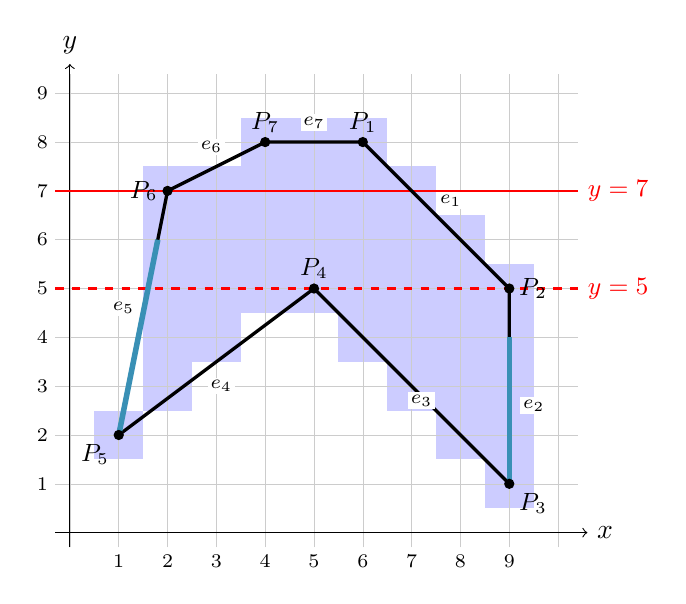
\begin{tikzpicture}[scale=0.62]
    \foreach \px/\py/\qx/\qy in {9/1/9/1, 1/2/1/2, 8/2/9/2, 2/3/2/3, 7/3/9/3, 2/4/3/4, 6/4/9/4, 2/5/9/5, 2/6/8/6, 2/7/7/7, 4/8/6/8}
        \fill[blue!20] (\px-0.5,\py-0.5) rectangle (\qx+0.5,\qy+0.5);
    \draw[step=1, gray!40, very thin] (-0.3,-0.3) grid (10.4,9.4);
    \draw[->] (-0.3,0) -- (10.6,0) node[right] {$x$};
    \draw[->] (0,-0.3) -- (0,9.6) node[above] {$y$};
    \foreach \i in {1,...,9} { \node[below, font=\scriptsize] at (\i,-0.25) {\i}; \node[left, font=\scriptsize] at (-0.25,\i) {\i}; }
    \draw[red, thick] (-0.3,7) -- (10.4,7) node[right] {\small $y = 7$};
    \draw[red, thick, dashed] (-0.3,5) -- (10.4,5) node[right] {\small $y = 5$};
    \draw[very thick] (6,8) -- (9,5) -- (9,1) -- (5,5) -- (1,2) -- (2,7) -- (4,8) -- cycle;
    \draw[cyan!70!black, line width=2pt] (1,2) -- (1.8,6);
    \draw[cyan!70!black, line width=2pt] (9,4) -- (9,1);
    \foreach \x/\y/\n/\pos in {6/8/P_1/above, 9/5/P_2/right, 9/1/P_3/below right, 5/5/P_4/above, 1/2/P_5/below left, 2/7/P_6/left, 4/8/P_7/above}
        \fill (\x,\y) circle (3pt) node[\pos, font=\small] {$\n$};
    \foreach \x/\y/\n in {7.8/6.8/e_1, 9.5/2.6/e_2, 7.2/2.7/e_3, 3.1/3.0/e_4, 1.1/4.6/e_5, 2.9/7.9/e_6, 5/8.4/e_7}
        \node[font=\scriptsize, fill=white, inner sep=1pt] at (\x,\y) {$\n$};
\end{tikzpicture}
\caption{Ví dụ tô màu đa giác theo dòng quét: đa giác $P_1 \ldots P_7$, các điểm ảnh được tô (ô xanh, với đoạn $[\lceil x_{2j-1}\rceil, \lfloor x_{2j}\rfloor]$), hai cạnh sau khi rút ngắn $e_5$, $e_2$ (nét xanh đậm) và hai dòng quét đặc biệt $y = 5$, $y = 7$}
\label{fig:w5_example}
\end{figure}

\textbf{Toàn bộ quá trình tô} theo giải thuật ET--AEL (mục~\ref{subsec:w5_ael}) với bảng cạnh ET[1] $= \{e_2: (4, 9, 0),\ e_3: (5, 9, -1)\}$, ET[2] $= \{e_4: (5, 1, \tfrac43),\ e_5: (6, 1, \tfrac15)\}$, ET[5] $= \{e_1: (8, 9, -1)\}$, ET[7] $= \{e_6: (8, 2, 2)\}$ (bộ ba \texttt{y\_upper}, \texttt{x\_int}, \texttt{reci\_slope})~\citep{dhmt_lec7}:
\begin{center}
\small
\renewcommand{\arraystretch}{1.2}
\begin{tabular}{|c|l|l|l|}
\hline
$y$ & \textbf{AEL đã sắp xếp (\texttt{x\_int})} & \textbf{Đoạn tô} & \textbf{Ghi chú} \\ \hline
1 & $e_2{:}\,9,\ e_3{:}\,9$ & $[9, 9]$ & $P_3$ cực tiểu: 2 giao điểm trùng \\
2 & $e_4{:}\,1,\ e_5{:}\,1,\ e_3{:}\,8,\ e_2{:}\,9$ & $[1, 1], [8, 9]$ & $P_5$ cực tiểu \\
3 & $e_5{:}\,\tfrac65,\ e_4{:}\,\tfrac73,\ e_3{:}\,7,\ e_2{:}\,9$ & $[2, 2], [7, 9]$ & \\
4 & $e_5{:}\,\tfrac75,\ e_4{:}\,\tfrac{11}{3},\ e_3{:}\,6,\ e_2{:}\,9$ & $[2, 3], [6, 9]$ & xóa $e_2$ (\texttt{y\_upper} $= 4$) \\
5 & $e_5{:}\,\tfrac85,\ e_4{:}\,5,\ e_3{:}\,5,\ e_1{:}\,9$ & $[2, 5], [5, 9]$ & thêm $e_1$; xóa $e_3, e_4$ \\
6 & $e_5{:}\,\tfrac95,\ e_1{:}\,8$ & $[2, 8]$ & xóa $e_5$ (đã rút ngắn) \\
7 & $e_6{:}\,2,\ e_1{:}\,7$ & $[2, 7]$ & thêm $e_6$; $P_6$ chỉ 1 giao điểm \\
8 & $e_6{:}\,4,\ e_1{:}\,6$ & $[4, 6]$ & xóa $e_6, e_1$; AEL rỗng, dừng \\ \hline
\end{tabular}
\end{center}

\subsection{Kỹ thuật Rút ngắn Cạnh tại các Đỉnh Không Cực trị trong Thuật toán Tô màu theo Dòng quét}
\label{subsec:w5_shorten}

Thuật toán tô màu đa giác theo dòng quét (Scan-line Polygon Fill Algorithm) hoạt động bằng cách cho dòng quét $y = y_{\text{scan}}$ quét tuần tự từ đáy lên đỉnh đa giác. Tại mỗi dòng quét, thuật toán tìm các giao điểm với các cạnh trong Bảng cạnh kích hoạt (Active Edge Table, AET), sắp xếp giao điểm theo hoành độ $x$ tăng dần, rồi tô màu các đoạn pixel nằm kẹp giữa từng cặp giao điểm lẻ và chẵn $(x_1, x_2), (x_3, x_4), \dots$ theo quy tắc chẵn lẻ.

\textbf{Vấn đề Xảy ra khi Dòng quét Đi qua Đỉnh Đa giác:}
Một đỉnh là giao điểm chung của hai cạnh kề nhau. Nếu dòng quét đi qua đỉnh, phép toán tìm giao điểm thông thường sẽ tìm thấy đỉnh đó hai lần (một lần trên mỗi cạnh), sinh ra hai giao điểm có tọa độ trùng nhau:
\begin{equation}
x_{\text{intersect}}^{(1)} = x_{\text{intersect}}^{(2)} = x_{\text{vertex}}
\end{equation}

Sự xuất hiện của hai giao điểm trùng nhau này có thể phá vỡ quy tắc Parity của toàn bộ các pixel phía sau trên dòng quét. Để xử lý chính xác, thuật toán phân loại đỉnh thành hai trường hợp bản chất:

\textbf{1. Đỉnh Cực trị Địa phương (Local Extremum gồm cực tiểu địa phương Local Minimum hoặc cực đại địa phương Local Maximum):}
Hai cạnh kề nhau của đỉnh cùng nằm về một phía của dòng quét (cùng nằm phía trên hoặc cùng nằm phía dưới, tức tung độ của hai đỉnh lân cận cùng lớn hơn hoặc cùng nhỏ hơn tung độ của đỉnh đang xét).
\begin{itemize}
    \item Khi dòng quét đi qua đỉnh cực trị, nó chỉ tiếp xúc với mép biên của đa giác mà không đi xuyên qua từ trong ra ngoài (hoặc ngược lại).
    \item Để bảo toàn quy tắc chẵn lẻ, đỉnh cực trị phải được tính là \textbf{hai giao điểm} (hoặc bỏ qua không tính). Khi được tính hai lần, tính chẵn lẻ không bị đảo lộn, các đoạn tô màu phía sau vẫn vận hành chính xác. Do đó, \textbf{giữ nguyên độ dài hai cạnh, không rút ngắn}.
\end{itemize}

\textbf{2. Đỉnh Không Cực trị (Non-extremum Vertex / Monotonic Vertex):}
Hai cạnh kề nhau của đỉnh nằm về hai phía đối lập của dòng quét: một cạnh đi lên phía trên và một cạnh đi xuống phía dưới.
\begin{itemize}
    \item Khi dòng quét đi qua đỉnh này, nó thực sự đâm xuyên từ miền ngoài vào miền trong đa giác (hoặc từ miền trong ra miền ngoài).
    \item Nếu tính cả hai cạnh, ta có 2 giao điểm (số chẵn), khiến thuật toán lầm tưởng dòng quét không đi xuyên qua biên, dẫn đến việc đảo ngược toàn bộ trạng thái tô màu của các pixel phía sau trên dòng quét đó (gây hiện tượng tràn màu ra ngoài hoặc mất màu bên trong).
    \item Vì vậy, đỉnh không cực trị bắt buộc chỉ được tính là \textbf{đúng một giao điểm duy nhất}.
\end{itemize}

\textbf{Giải pháp Kỹ thuật: Rút ngắn Cạnh (Edge Shortening):}
Để đảm bảo đỉnh không cực trị chỉ tạo ra đúng 1 giao điểm khi dòng quét đi qua, thuật toán chuẩn hóa quy ước rút ngắn một trong hai cạnh kề đi đúng 1 đơn vị tung độ:
\begin{equation}
y_{\max} = y_{\max} - 1 \quad \text{(đối với cạnh nằm phía dưới đỉnh)}
\end{equation}
hoặc:
\begin{equation}
y_{\min} = y_{\min} + 1 \quad \text{(đối với cạnh nằm phía trên đỉnh)}
\end{equation}
Nhờ việc rút ngắn cạnh này, tại dòng quét đi qua đỉnh, chỉ có duy nhất một cạnh chứa đỉnh đó còn nằm trong Bảng cạnh kích hoạt AET, đảm bảo số giao điểm luôn được ghi nhận là một số lẻ khi xuyên qua biên, giúp thuật toán Scan-line Fill tô màu chính xác $100\%$ không gian đa giác mà không gặp lỗi tràn biên.

% ===== added from week04-huy =====
\subsection{Ý nghĩa từng trường trong cấu trúc AEL}
\label{subsec:w5_ael}

\textit{Câu hỏi: Giải thích mỗi trường trong cấu trúc dữ liệu AEL (Active Edge List) của thuật toán tô màu theo dòng quét.}

Cấu trúc AEL được định nghĩa như sau~\citep{dhmt_lec7}:
\begin{verbatim}
struct AEL {
    int   y_upper;     // tung do lon nhat cua canh (sau khi da rut ngan)
    float x_int;       // hoanh do giao diem voi dong quet hien tai
    float reci_slope;  // nghich dao he so goc: 1/m = dx/dy
    struct AEL *next;  // con tro toi canh ke tiep trong danh sach
};
\end{verbatim}
\begin{itemize}
    \item \texttt{y\_upper}: dòng quét cuối cùng mà cạnh còn cắt. Khi dòng quét $y$ vượt quá \texttt{y\_upper}, cạnh bị loại khỏi danh sách. Đây là trường nhận kết quả của việc rút ngắn cạnh ($y_i - 1$) ở mục~\ref{subsec:w5_shorten}. Lưu dạng số nguyên vì dòng quét là số nguyên.
    \item \texttt{x\_int}: hoành độ giao điểm (intersection) của cạnh với dòng quét đang xử lý. Khi cạnh được đưa vào AEL, giá trị khởi tạo là hoành độ đầu dưới của cạnh. Sau mỗi dòng quét được cập nhật tăng dần. Lưu số thực vì giao điểm thường không nguyên; khi tô thì làm tròn (đầu trái làm tròn lên, đầu phải làm tròn xuống) để không tô ra ngoài biên.
    \item \texttt{reci\_slope}: $1/m = \Delta x / \Delta y$. Khi dòng quét tăng $1$ thì $x$ trên cạnh tăng đúng $1/m$, nên \texttt{x\_int += reci\_slope}: tính giao điểm mới chỉ bằng một phép cộng, không cần giải lại phương trình đường thẳng (cùng tư tưởng gia số như phương pháp gia số ở mục~\ref{subsec:w4_dda}). Dùng nghịch đảo hệ số góc thay vì $m$ vì cạnh thẳng đứng có $1/m = 0$ hợp lệ, còn cạnh nằm ngang ($m = 0$) đã bị loại khỏi danh sách.
    \item \texttt{next}: danh sách liên kết, vì số cạnh hoạt động thay đổi liên tục (thêm cạnh mới khi dòng quét chạm đầu dưới, xóa khi vượt đầu trên). Danh sách được giữ \emph{sắp xếp theo} \texttt{x\_int} tăng dần để bước L4 ghép cặp lẻ--chẵn trực tiếp. Do các cạnh trong đa giác đơn không cắt nhau, thứ tự này ít thay đổi giữa hai dòng liên tiếp, nên sắp xếp chèn (insertion sort) gần như $O(k)$.
\end{itemize}

\textbf{AEL trong toàn bộ thuật toán.} AEL đi kèm bảng cạnh ET (Edge Table), được khai báo là \texttt{struct AEL *ET[MAX\_LINES]}: phần tử $ET[y]$ trỏ tới danh sách các cạnh có \emph{đỉnh thấp} (đầu dưới) nằm trên dòng quét $y$; mỗi phần tử dùng cùng cấu trúc trên, với \texttt{x\_int} khởi tạo bằng hoành độ đầu dưới. ET được lập sau bước tinh chỉnh dữ liệu (bỏ cạnh song song $Ox$, rút ngắn cạnh tại đỉnh không cực trị). Giải thuật tô màu dựa trên ET và AEL~\citep{dhmt_lec7}, với con trỏ \texttt{Beglist} trỏ tới đầu danh sách AEL:
\begin{enumerate}[label=L\arabic*.]
    \item Lặp với mỗi dòng quét $y$ từ \texttt{MIN\_Y} đến \texttt{MAX\_Y}:
    \item \quad nếu $ET[y] \ne$ \texttt{NIL} thì
    \item \quad\quad thêm các cạnh do $ET[y]$ trỏ tới vào AEL (\texttt{Beglist});
    \item \quad nếu \texttt{Beglist} $\ne$ \texttt{NIL} thì: sắp xếp AEL theo \texttt{x\_int} tăng dần; tô các điểm ảnh giữa từng cặp giao điểm lẻ--chẵn trên dòng $y$; xóa khỏi AEL các cạnh có \texttt{y\_upper} $= y$; cập nhật \texttt{x\_int += reci\_slope} cho các cạnh còn lại.
\end{enumerate}
Bảng ở mục~\ref{subsec:w5_scan7} cho thấy trạng thái AEL qua từng dòng quét của ví dụ. Thứ tự ``xóa rồi mới cập nhật'' quan trọng: cạnh có \texttt{y\_upper} $= y$ vẫn tham gia tô ở dòng $y$, rồi mới bị loại, nên đầu trên của cạnh không bị mất.

\textbf{Nhận xét.} ET là cấu trúc sắp xếp theo thùng (bucket sort) theo $y$, AEL là danh sách động theo $x$. Hai cấu trúc này biến bài toán ``tìm giao điểm của mọi cạnh với mọi dòng quét'' ($O(\text{số cạnh} \times \text{số dòng})$) thành chỉ xử lý các cạnh đang hoạt động, mỗi bước một phép cộng. Đây là ví dụ điển hình của việc khai thác \emph{tính liên kết} (coherence) giữa các dòng quét liên tiếp trong hệ thống đồ họa.
